\documentclass{article}
\usepackage[utf8]{inputenc}
\usepackage[margin=0.8in]{geometry}
\usepackage{graphicx}
\usepackage{algorithm}
\usepackage{algorithmicx}
\usepackage[noend]{algpseudocode}
\usepackage{tikz}
\usetikzlibrary{calc, shapes.multipart, chains, arrows, positioning}
\tikzstyle{vertex}=[draw, fill=myseagreen, circle, minimum
size=21pt, inner sep=0pt]
\tikzstyle{splitvertex}=[draw, fill=myseagreen,circle split, minimumsize=21pt]

\definecolor{myseagreen}{RGB}{238,238,238}
\definecolor{mysalmon}{RGB}{204,204,204}
\definecolor{mypurple}{RGB}{170,170,170}
\definecolor{myblack}{RGB}{0,0,0}
\definecolor{mywhite}{RGB}{255,255,255}

\title{Trees}
\author{George Tang}
\date{5 October 2018}

\begin{document}

\maketitle

\section{Definitions}
A tree is a special type of graph that satisfies two constraints:
\begin{itemize}
    \item All nodes must be connected by edges.
    \item There are no \textit{cycles}, a set of distinct edges that can be followed from any node to reach itself.
\end{itemize}

\begin{figure}[h]
\centering
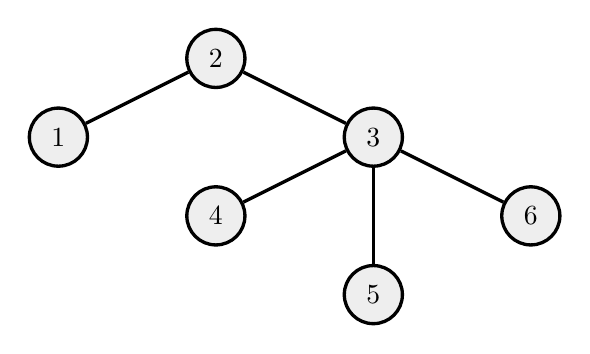
\begin{tikzpicture}[very thick,level/.style={sibling distance=70mm/#1}]
\draw (0, 0) node [vertex] (n1) {1};
\draw (2, 1) node [vertex] (n2) {2};
\draw (4, 0) node  [vertex] (n3) {3};
\draw (2, -1) node [vertex] (n4) {4};
\draw (4, -2) node [vertex] (n5) {5};
\draw (6, -1) node [vertex] (n6) {6};
\draw (n1) -- (n2);
\draw (n2) -- (n3);
\draw (n3) -- (n4);
\draw (n3) -- (n5);
\draw (n3) -- (n6);
\end{tikzpicture}
\caption{This diagram illustrates a tree.}
\end{figure}

Every node c except the \textit{root} is connected to some other node p called the \textit{parent} of c. We also call c the \textit{child} of p. Nodes that have no children are called \textit{leaves}. The \textit{ancestors} of a node are all the nodes on the path between it and the root.  

\section{Implementation}
There are two ways to implement a tree data structure:
\begin{itemize}
    \item Nodes are defined as a class with a list of children, pointer to parent, and the data it holds.
    \item Node information are stored in many arrays (parent, children, data), where the index corresponds to the node id. For the children array, each index holds a linked list of children node ids. This one is the favorite of competitive programmers.
\end{itemize}

\section{Traversals}
There are three types of tree traversals. Each traversal is recursive, meaning you repeat the traversal until you reach a leaf node or all children have been visited
\begin{itemize}
    \item \textit{Preorder}: visit the current node first, then the children nodes.
    \item \textit{Postorder}: visit all children nodes then the current node.
    \item \textit{Inorder}: when there are only two children, and the child with a smaller data (or equal to) value than the current node's data value is the left child, and the child with the larger value is the right child. Visit the left node, then then current node, and then the right node.

\end{itemize}

\section{Binary Search Trees}
A binary tree has only two children. In the inorder traversal section, we introduced a binary search tree. BSTs are often very useful in contest, especially when there requires a $logN$ search query on an enumerable data set. However this requires the BST to be \textit{balanced}, meaning that the left and right subtrees of the current node are not too different in size. This occurs when the data is inserted in random order. Once we cover insertion, convince yourself this is tree. For the following implementations, we assume the array representation (left refers to child[0] and right child[1]). The tree representation can be easily extended from the following.    

\subsection{Search}
\begin{algorithm}[H]
\caption{BST Search}
\begin{algorithmic}
\Function{Search}{$curr$, $u$}
    \If {$curr.val = u$}
		\State \Return $curr$
	\EndIf
	\If {$curr.left = null$ and $curr.right = null$}
	    \State \Return $null$
	\EndIf
    \If{$curr.val < u$}
        \State \Return \Call{SEARCH}{$curr.left$, $u$}
    \Else
    	\State \Return \Call{SEARCH}{$curr.right$, $u$}
    \EndIf
\EndFunction
\end{algorithmic}
\end{algorithm}

\subsection{Insert}
\begin{algorithm}[H]
\caption{BST Insert}
\begin{algorithmic}
\Function{Insert}{$curr$, $u$}
    \If {$curr.val =< u$}
        \If{$curr.left = null$}
            \State $curr.left$ = Node($u$)
        \Else
            \State \Call{INSERT}{$curr.left$, $u$}
        \EndIf
    \Else
        \If{$curr.right = null$}
            \State $curr.right$ = Node($u$)
        \Else
            \State \Call{INSERT}{$curr.right$, $u$}
        \EndIf
    \EndIf

\EndFunction
\end{algorithmic}
\end{algorithm}

\subsection{Delete}
Three cases for node to be deleted:
\begin{itemize}
    \item no children
    \item one child
    \item two children
\end{itemize}

\begin{algorithm}[H]
\caption{BST Delete}
\begin{algorithmic}
\Function{minnode}{$curr$}
    \While{$curr.left$ != null}
        \State $curr$ = $curr.left$
    \EndWhile
    \State \Return $curr$
\EndFunction
\Function{Delete}{$node$, $u$}
    \If{$node.left = null$ and $node.right = null$}
        \State $node$ = $null$
    \EndIf
    \If{$node.left != null$ and $node.right != null$}
        \State $temp$ = \Call{minnode}{$node$}
        \State $node.val$ = $temp.val$
        \State $temp$ = $null$
    \Else
        \If{$node.parent.left = node$}
            \If{$node.left = null$}
                \State $node.parent.left$ = $node.right$
            \Else
                \State $node.parent.left$ = $node.left$
            \EndIf
        \Else
            \If{$node.left = null$}
                \State $node.parent.right$ = $node.right$
            \Else
                \State $node.parent.right$ = $node.left$
            \EndIf
        \EndIf
    \EndIf

\EndFunction
\end{algorithmic}
\end{algorithm}
\subsection{Lazy Delete}
If memory is not an issue, you can just keep a flag that indicates whether the node has been deleted or not. 

\section{Problems}
\subsection{USACO Gold February 2018, Cow at Large}
The farm consists of (2 $\leq N \leq 10^5$) barns and $N-1$ bidirectional tunnels. Every barn is connected. Every barn with one tunnel is an exit. Bessie will be at any barn and attempt to exit. The moment Bessie starts walking, farmers will start at various exit barns and attempt to catch Bessie. The farmers and Bessie can traverse one edge per unit time. Everyone knows where everyone else is at all times. The farmers catch Bessie if at any instant a farmer is in the same barn as Bessie, or crossing the same tunnel as Bessie. Given that Bessie starts at barn K, help Bessie determine the minimum number of farmers needed to catch Bessie.

\end{document}
